% \documentclass[12pt,openright,oneside,a4paper,brazil]{abntex2}
% \usepackage[utf8]{inputenc}
% \counterwithout{section}{section}
% \counterwithout{figure}{chapter}
% \counterwithout{table}{chapter}
% \setlength{\parindent}{1.3cm}
% \usepackage{indentfirst}
% \setlength{\parskip}{0.2cm}
% \usepackage[bottom=2cm,top=3cm,left=3cm,right=2cm]{geometry}
% \usepackage{graphicx}
% \graphicspath{{figuras/}}
% \usepackage{placeins}
% 
% %opening
% \title{}
% \author{}
% 
% \begin{document}
% 
% 
% \textual
\begin{center}
 {\large Plano de gerenciamento dos Recursos Humanos}\\[0.2cm]
 {Planta de abastecimento de água potável a partir da umidade do ar}\\
 \end{center}
 
 \section*{Histórico de Alterações}
\begin{table}[h]
\centering
\begin{tabular}{|c|c|p{7cm}|c|}

Data & Versão & Descrição & Responsável\\
\hline                               
19/04/2015 & 0.0 & Criação do plano de recursos humanos e suas especificações. & Amanda Leite de Castro\\
\hline
\end{tabular}
\end{table}

\section*{Objetivo}
  O objetivo desse plano é estabelecer um processo de gerenciamento dos recursos humanos do projeto.
  
  \section*{Perfil dos recursos humanos}
  \begin{itemize}
   \item Gerente de Projeto – Adrianny Viana de Araújo Amorim: responsável pelo projeto; realizar a gestão da mudança, escopo, custo, qualidade e os recursos que serão compartilhados entre os vários setores do projeto; selecionar e adaptar os processos de gerenciamento de projetos mais apropriados para a realidade da gerência, na medida da necessidade; dirigir e liderar a equipe, almejando a realização dos objetivos e metas; acompanhar a maturidade da equipe em gerenciamento de projetos, identificando necessidades de orientação e treinamentos; aprovar o plano de cada parte do projeto e autoriza sua execução; definir documentos padrões, base de dados e ferramentas; convocar e coordenar reuniões do projeto; administrar conflitos; definir o escopo do produto.
   \item Gerente setorial: responsável por gerenciar as equipes definidas por áreas de desenvolvimento; definir requisitos de qualidade do produto; responder pela licitação e documentação de requisitos; garantir as entregas dos pacotes de trabalho; acompanhar o desempenho e a elaboração do produto; subordinado ao gerente de projetos, responsável por relatar o andamento do projeto a este.\\
Componentes:\\
Gerente de Escopo – Ítalo Paiva Batista\\
Gerente de Qualidade – Alexandre Torres Kryonidis\\
Gerente de Tempo – Hugo Ferreira Martins\\
Gerente de Integração – Laís Rocha Carvalho \\
Gerente de Custos – João Gabriel da Silva Souza\\
Gerente de Comunicação – Vítor Ferreira Pacífico \\
Gerente de Riscos – César Antônio Marques Junior \\
Gerente de Aquisições – Yan Watanabe Martins\\
  \item Grupo de Suporte à Decisão – fornece recursos humanos para o projeto; auxilia na definição do escopo, na elaboração dos planos e na avaliação de solicitações de mudança.\\
  Componentes: \\
  Amanda de Leite Castro;\\
  Eric Vinicius Lima Barbosa;\\
  Júlio César Tavares Primo.\\
  \item Equipe: identifica e informa as necessidades de mudanças; informa a ocorrência de contingências que podem impactar no insucesso do projeto; registra e arquiva as atividades, documentos elaborados e lições aprendidas; entregar formalmente (com aceitação) os pacotes de trabalho.\\
Componentes:\\
Ana Paula Chavier Rodrigues;\\
Andre Luis Motoshima Barros;\\
Brenda Tagna Cardoso Pinheiro De Paula;\\
Filippe Henriques Leal;\\
Guilherme Pfeilsticker De Oliveira Matias Pereira;\\
Gustavo Henrique De Souza Pereira;\\
Jonnatas Lennon Lima Costa;\\
Karine Santos Valença;\\
Ludimila Soares Ferreira;\\
Matheus Jerico Palhares;\\
Pedro Kelvin De Castro Moreira Batista;\\
Rafael Abreu De Carvalho;\\
Rafael Contessotto Braganca Pinheiro;\\
Victor Felipe Borges;\\
Vitor Silva Ribeiro.\\
  \end{itemize}
\newpage
\section*{Organograma do Projeto}
  \begin{figure}[!ht]
\centering
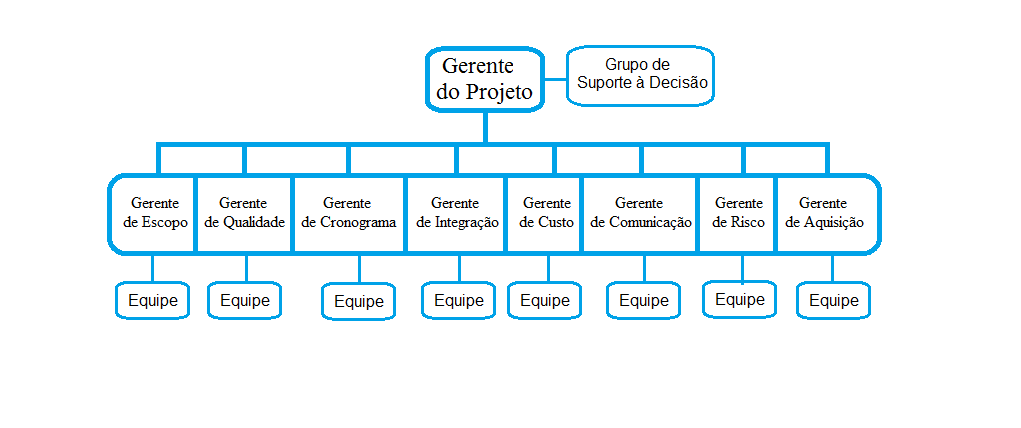
\includegraphics[scale=0.6]{editaveis/figuras/Organograma}
\caption{Organograma do projeto}
\label{Organograma}
\end{figure}

\FloatBarrier
\begin{figure}[!h]
      \centering
      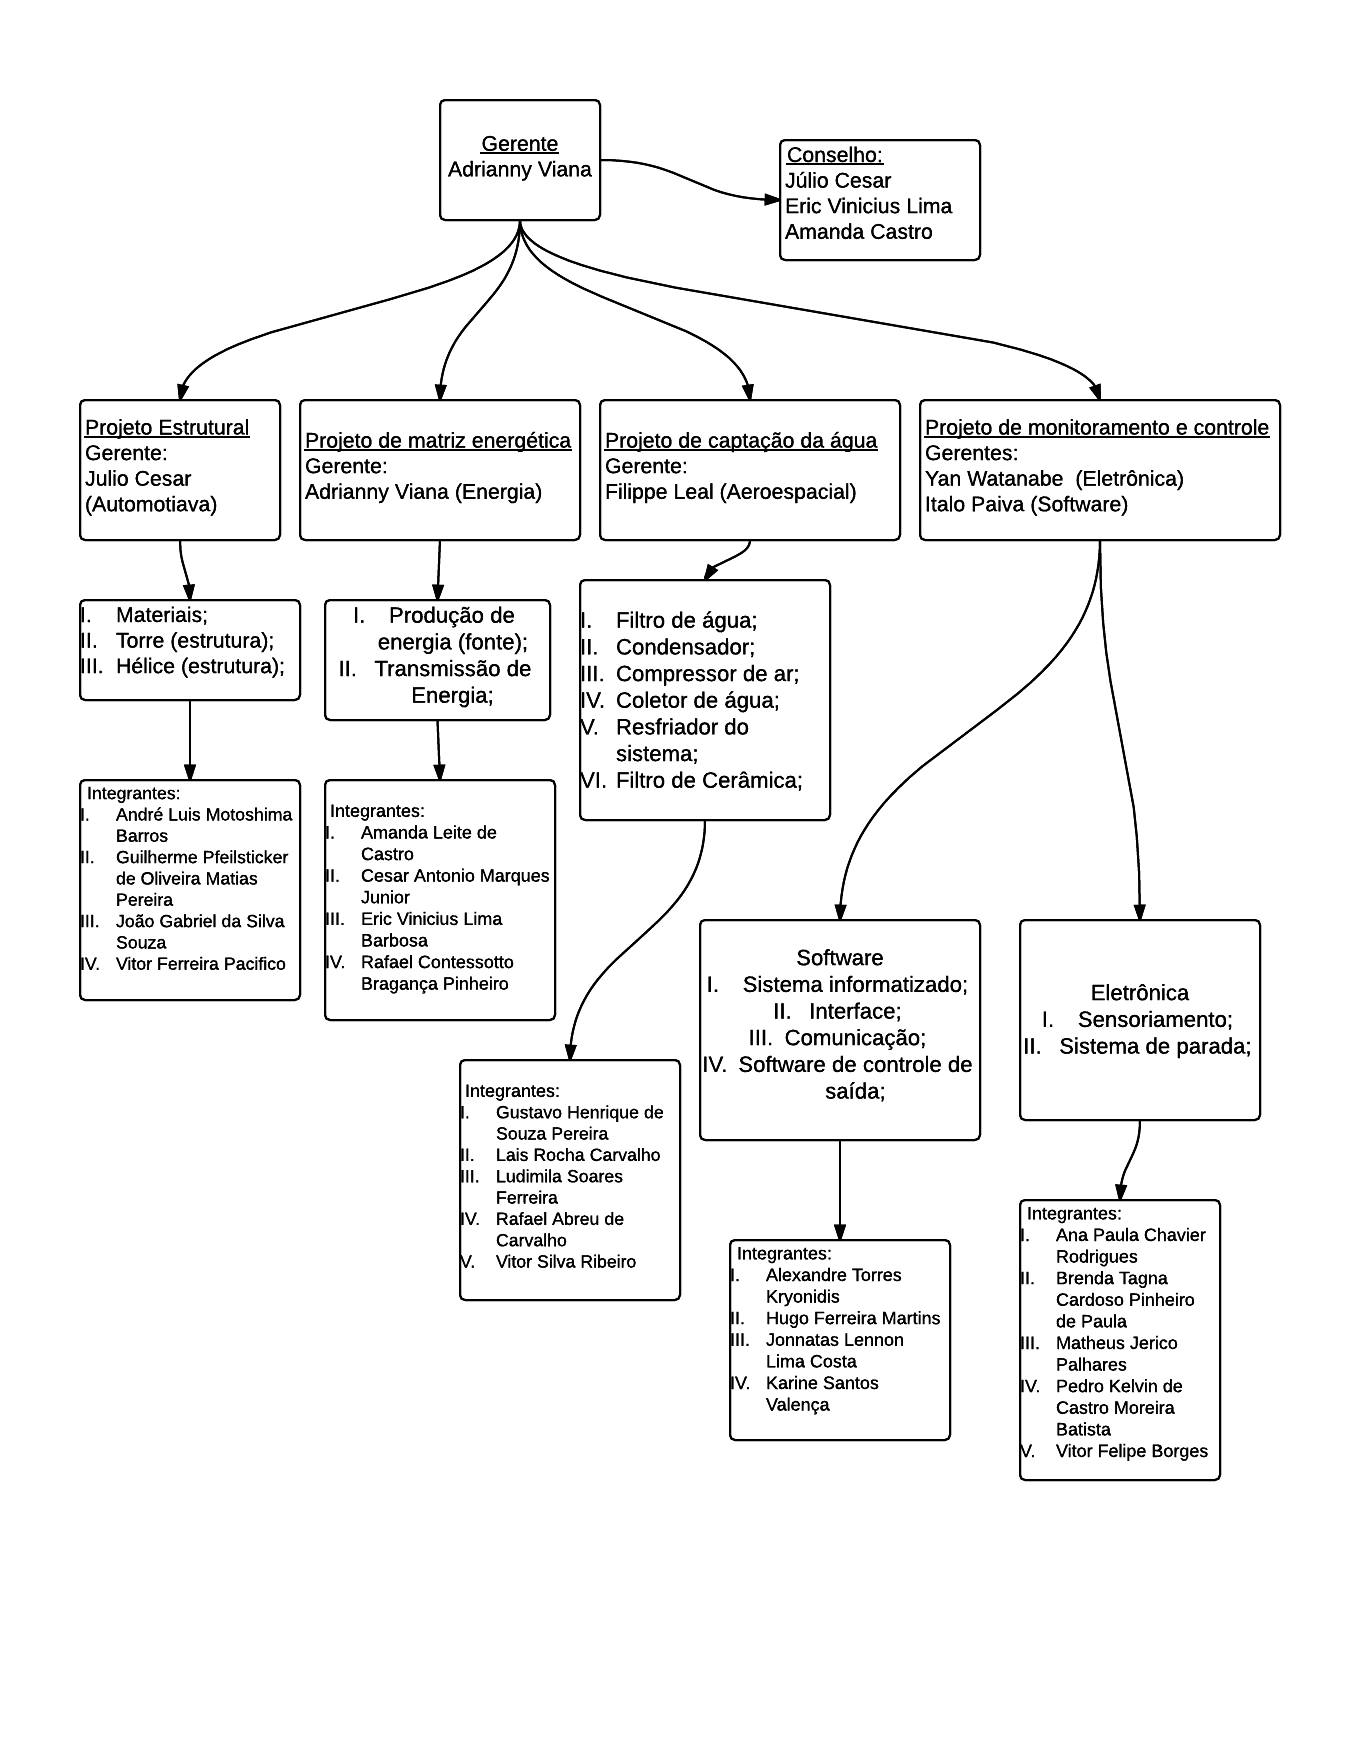
\includegraphics[scale = 0.27]{editaveis/figuras/Fluxograma_gerencia}
      \label{fluxograma_gerencia_projeto}
      \caption{Fluxograma da gerência do projeto}
    \end{figure}
    \FloatBarrier

 \section*{Matriz de Responsabilidades}
 \FloatBarrier
 \begin{figure}[h]
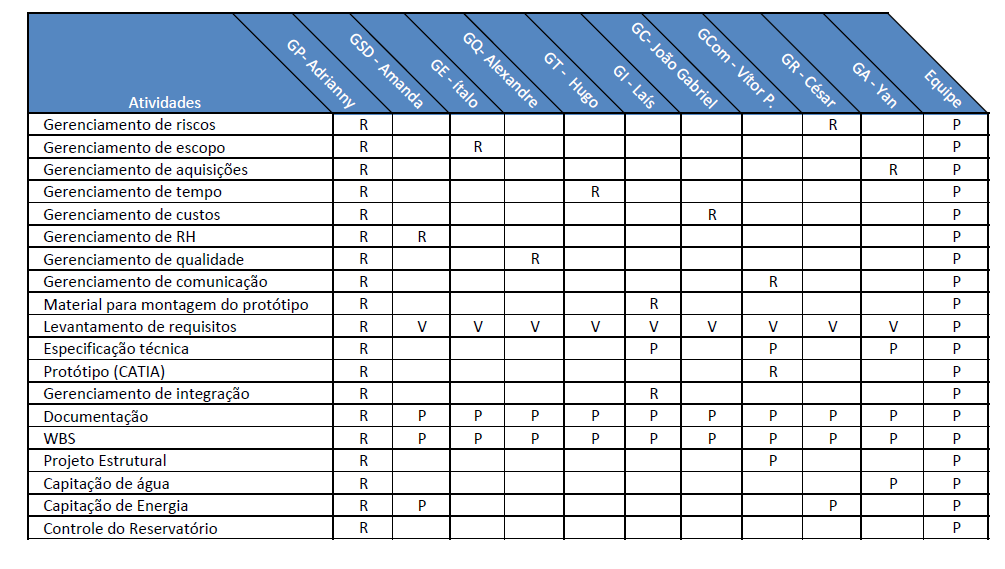
\includegraphics[scale=0.65]{editaveis/figuras/matriz}
\label{matrizderesponsabilidades}
\caption{Matriz de Responsabilidades}
 \end{figure}

Legenda: R= Responsável; V= Valida; P= Participa.\\
  

\section*{Novos recursos, realocação e substituição dos membros do time}
Em busca da realização dos objetivos do projeto, o gerente dos recursos humanos tem a responsabilidade e autoridade total para gerenciar e manejar todo o projeto, observando todo o ciclo de vida do mesmo, com o propósito de executar uma adequada alocação, realocação e substituição de recursos humanos, ou diversos, através do reconhecimento de competências, seleção, monitoração da alocação e avaliação dos recursos disponíveis ao projeto.

\section*{Treinamento}
\begin{itemize}
 \item Capacitação da equipe do projeto: treinamento sobre Fundamentos de Gerenciamento de Projetos, onde deve ser abordada uma visão geral da metodologia, ferramenta, prática e cultura de gerenciamento de projetos.

 \item Desenvolvimento da tecnologia: treinamento interativo com o pessoal de produção, durante o qual se cria e desenvolve as instruções técnicas e de qualidade designadas. Consiste em apresentar um projeto de protótipo sobre a tecnologia utilizada no processo.

  \item Gestão da população de Acari: treinamento para capacitação de pessoal que interaja com a população e seus respectivos representantes políticos.
\end{itemize}

É de plena responsabilidade do Departamento de Recursos Humanos analisar as falhas de competência dos componentes do time verificados por meio das avaliações de desempenho para desenvolver treinamentos de qualificação e aperfeiçoamento.

\section*{Avaliação de resultados do time do projeto}
Os sistemas de avaliação dos resultados do time do projeto são feitos a partir de reuniões semanais, nas quais são demonstradas e discutidas as evoluções até então, como também são definidos os próximos passos a serem dados, com base nas determinações já realizadas e nas orientações do que necessita ser feito.

\section*{Bonificação}
Caso o projeto seja entregue em prazo estipulado e atendendo todos os requisitos de qualidade, a equipe do projeto receberá uma gratificação. O time terá uma confraternização social ao final do projeto.

\section*{Freqüência da avaliação consolidada dos resultados do time}
Os resultados da frequência de avaliação serão apresentados em reuniões com o time, e divulgados nas plataformas de comunicação objetivando o esclarecimento de todos da equipe. Porém, haverão questões a serem discutidas individualmente com cada integrante do time.

\section*{Alocação financeira para o gerenciamento de recursos humanos}
No gerenciamento de Recursos Humanos, os gastos adicionais relacionados ao setor devem ser alocados dentro das reservas gerenciais do projeto, sendo os responsáveis por administrar tais reservas os Gerentes de Projeto.

\section*{Administração do plano de gerenciamento de recursos humanos}
\begin{enumerate}
 \item Responsável pelo plano:\\
 AMANDA LEITE DE CASTRO - GERENTE DE SUPORTE Á DECISÃO

ERIC VINÍCIUS LIMA BARBOSA - SUPLENTE DO RESPONSÁVEL DIRETO PELO PLANO DE GERENCIAMENTO DE SUPORTE À DECISÃO.
  \item Frequência de atualização do plano de gerenciamento de recursos humanos:\\
  O Plano de Gerenciamento de Recursos Humanos será revisto em reunião, datada para o dia 20/04/2015, e em suas reuniões subsequentes determinando e avaliando os resultados de cada membro do time.
\end{enumerate}

\section*{Outros assuntos relacionados ao gerenciamento de recursos humanos do projeto não previstos nesse plano}
Todas as mudanças no quadro de gerenciamento dos Recursos Humanos devem ser apresentadas e discutidas em reunião sendo o Gerente de Recursos Humanos o responsável por tal avaliação. A responsabilidade de possíveis mudanças no quadro pessoal da equipe fica direcionada à comissão.

\section*{Assinaturas}
\begin{center}
Data: \rule{0.5cm}{0.1mm}/\rule{0.5cm}{0.1mm}/\rule{1cm}{0.1mm}     \\
\rule{13cm}{0.1mm}\\
ADRIANNY VIANA DE ARAÚJO AMORIM – GERENTE DE PROJETO\\
\rule{13cm}{0.1mm}\\
AMANDA LEITE DE CASTRO - GERENTE DE RECURSOS HUMANOS

\end{center}
% \end{document}